\documentclass{seal_article}

\usepackage{hyperref}
\usepackage{booktabs}
\usepackage{float}
\usepackage{caption}
\usepackage{subcaption}

\title{Bug prediction \& ASAT adoption \\in Cloud Applications}
\subtitle{Paper for the Software Maintenance \& Evolution course \\ Anna Jancso, Yasara Peiris, Sophy Chhong}

\begin{document}
\maketitle

\section{Introduction}
Cloud computing has become backbone of computing  with the increase complexity of modern software systems due to large code bases, more dependencies, more instances and more users. In this context, software evolution and maintenance has become more challenging with the increase of complexity for adding new features and difficulties in maintaining the code. 
In the meantime, bug prediction also plays a major role in the context of maintaining code. Different models and techniques have been presented for software defect prediction of traditional software projects which lead to make significant performance improvement in software maintenance. But due to the change of higher level architecture, existing prediction tool approach couldn’t reach to higher performance as earliar.

\section{Related Work}
A study related to proposing better algorithm for prediction model to predict future software faults based on historical data was done by investigating 3 main machine learning techniques, which are Naïve Bayes, Decision Tree and Artificial Neural Network. Evaluation process was carried out using three real testing/debugging datasets and results were collected based on basic measures, which are accuracy, precision recall and Relative mean squared error. Results revealed that Machine Learning approach is the best algorithm comparison to other algorithms in the context of defect prediction using historical data. \cite{hammouri}

A study of investigating bugs in distributed system was carried out by researchers in the past for the benefit of cloud research community by focusing on six popular and important scale-out systems: Hadoop, HDFS,HBase, Cassandra, ZooKeeper, and Flume, which collectively represent a diverse set of scale out architectures. They  have shared their high-level findings on different types of bugs that require more attention for future researches. the most useful object oriented features were found out as CBO, RFC and LOC while the most commonly used feature selection technique was identified as correlation-based feature selection. \cite{gunawi}

In addition to the previous works, a study showed modification for change metrics improve the performance of fault predictors complement to the static code metrics. Experiments carried out were shown that new metrics  provide an improve increase in recall, approximately 10 percent over the static code metrics  while modification to the change metrics improved the performance of the model approximately two or three percent over existing change metrics.\cite{choudhary}

Recent studies have proposed a parallel hybrid wrapper-filter approach to find out key software metrics for efficient identification of software module as defect or not. Proposed approach which is a combination of multiple filters with a wrapper were extensively analysed through various type of real defect-prone data sets for the robust evaluation.
\cite{ali}

Recent study was explored new type of cloud computing which is “Desktop Cloud” with an aim of reducing cost. The aim of this desktop cloud was to provide Cloud services out of infrastructure. In that context this paper carried out an experiment on studying the impact of node failures using evaluation metrics based on real data. Analysis of failure events in cloud environment and contribution to future research studies were done through proposing metrics to evaluate desktop computing. \cite{alw}






\section{Methodology}

In this Section, we describe how we proceeded in answering the the two research questions.

\subsection{Bug prediction}
The study aims to analyse the performance accuracy of cloud specific bugs using traditional bug prediction pipeline. 

\subsubsection{Project Sample}
Since we used the tool \textsc{ck} \cite{ck} to compute some of our metrics which specifically targets \textsc{Java} projects, we only included Java cloud projects in our sample. Furthermore, we selected projects with at least 100 releases.



\subsubsection{Data Preparation}
\paragraph{\textit{Metrics Selection}}
Important metrics types to feed in to bug prediction pipeline were chosen based on earlier researches on similar context. The following metrics are traditional CK metrics, used in detecting traditional software bugs. \cite{ck}

\begin{itemize}
\item loc - Counts the lines of code ignoring the empty lines.
\item cbo - Counts the number of dependencies of each class 
\item dit -  Counts the inherited classes of each class
\item wmc - Counts the number of branch instructions in a class
\item lcom - Lack of cohesion of methods
\end{itemize}

Investigation in using other kind of metric, i.e. number of microservices, has been done. Needed was a dynamic check of a running project to observe metrics like microservices. No dynamic checks were used in our experiments.

\paragraph{\textit{Data Ingestion}}
JGit is a java implementation of Git version control system. Git parser was implemented as the initial step of the bug prediction pipeline. All the commit messages between 2 releases were retrieved through the parser and then bug related commits were filtered using specific keywords to filter out the class names with the bugs.
\\Keywords to filter bugs : 
\textit{error, fix, failure, crash, unexpected, wrong}
\vspace{\baselineskip}
\textsc{CK} \cite{ck} library was used in for all the classes at the time of the release in order to retrieve the certain features to generate the metrics. CK java library provides class level and metric level code metrics without compiling the code. Above mentioned loc, cbo, dit, wmc, lcom were calculated written into the excel sheet with an extra column mentioning whether each of the class has a bug or not by going through the list of class names with bugs.

\paragraph{\textit{Data Cleaning}}
Data duplication could not be handled at the level of the java code due to the limitations of the used libraries. Before feeding in to the machine learning pipeline quality and reliability of data was assured through various pre-processing steps. In this stage irrelevant and redundant data is removed. 

\subsubsection{Process Diagram}
\vspace{\baselineskip}
\begin{figure}[htp]
    \centering
    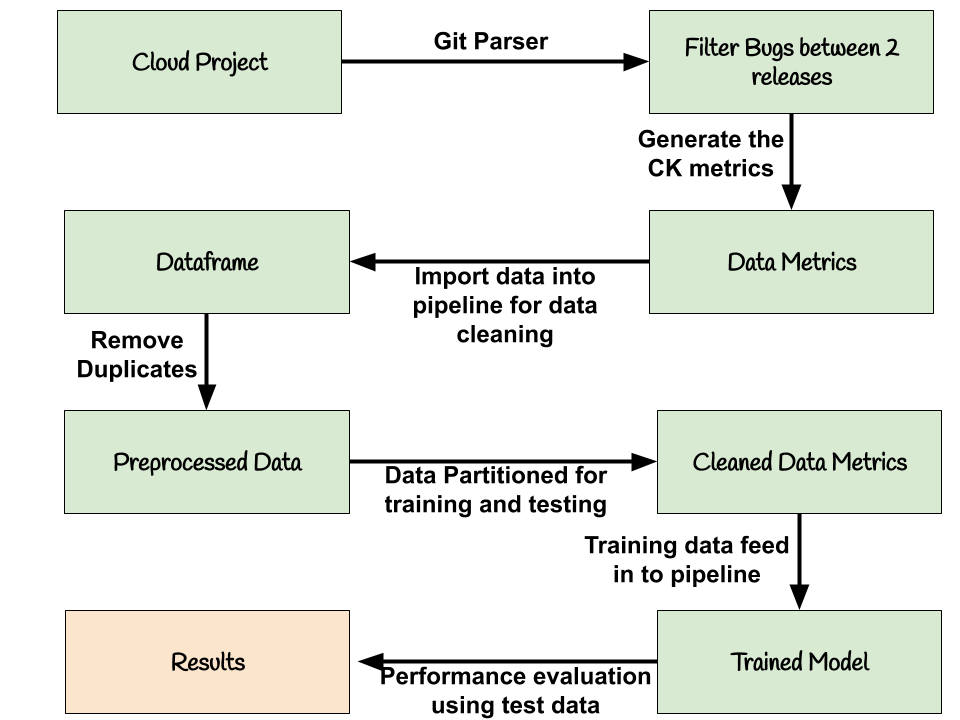
\includegraphics[width=8cm]{Process.png}
    \caption{Machine Learning Pipeline}
    \label{fig:Initial Bug }
\end{figure}

\subsubsection{Experimental Results}
Experiment was performed on Python Weka Machine Learning Platform. Naive Bayes, random forest and logistic regression were used as the machine learning algorithm. For the performance evaluation following metrics were used. Precision (P), Recall (R) and F-Measure (F).
All the metrics evaluations done on class level. Following equations were used for above evaluations.

In the context of the work, precision is calculated by dividing number of correctly classified defective classes to total number of defective classes.
\[ Precision = True Positive /(False Positive + True Positive)  \]

In the context of the work, Recall is calculated by dividing the number of defected classes to total number of defective modules.
\[ Recall = True Positive /(False Negative + True Positive) \]

F measure is defined as the weighted harmonic mean of the 
precision and recall. 
\[ F Score = 2 / ((1/recall)+(1/precision)) \]

10 fold cross validation technique was used used for the experiment.

\subsection{ASAT adoption in Cloud System}
To answer RQ2, we took the following steps:
\begin{itemize}
    \item We collected all ASATs available for the Go language.
    \item We classified the ASATs.
    \item We compiled a sample of cloud and non-cloud projects.
    \item We extracted ASAT usage in the projects.
\end{itemize}

\subsubsection{ASATs}
There are almost 50 ASATs available for the Go language. We mainly gathered these tools from a GitHub repository \cite{awesome_asat} that compiles a list of ASATs for many programming languages. We excluded some of these tools, namely those that were archived or deprecated (e.g. \cite{interfacer}), or exploratory in nature (e.g. \cite{goroutine}) as we were interested in ASATs highlighting issues in the code. We stored all ASATs in a sqlite database.

The majority of ASATs specialize on specific problems in the code such as detecting deadlocks \cite{dingo-hunter} or unused arguments in function declarations \cite{nargs}. Two ASATs in our database are linter aggregators , i.e. they run multiple ASATs \cite{goreporter,golangci-lint}. Finally, some ASATs cover a variety of code issues (e.g\cite{staticcheck}). 

Many ASATs can be configured in terms of which warnings are enabled, what files they are run on or at which thresholds a warning should be issued. These configuration settings may be passed via a file or command line arguments.

\subsubsection{Classification of ASATs}
We classified the linters into four categories: readability, efficiency, correctness and security. Readability linters aim to flag code fragments that are harder to understand due to code style issues, misspellings or lengthy functions. Efficiency linters aim to improve speed and memory usage. Correctness linters aim to find errors. Security linters aim to find vulnerabilities. ASATs not used in any project or not fitting in any of the categories (e.g. linter aggregators) are dropped for lack of space (in the former case their classifications are available in the database): \\

\noindent \textbf{Readability}:
\begin{itemize}
    \item wsl (enforcing empty lines at the right places)
    \item whitespace (unnecessary new lines)
    \item nakedret (unused function arguments)
    \item misspell (misspelled words)
    \item lll (file line length)
    \item gosimple (simplifying code)
    \item golint (coding style issues)
    \item gofmt (code formatting)
    \item gocyclo (cyclomatic complexities)
    \item goconst (Repeated strings that could be replaced by a constant)
    \item flen (function length)
    \item errcheck (error return values)
    \item dupl (duplicated code)
\end{itemize}

\noindent \textbf{Efficiency}:
\begin{itemize}
    \item varcheck (unused global variables and constants)
    \item unused (unused constants, variables, functions and types)
    \item unconvert (unnecessary type conversions)
    \item structcheck (unused struct fields)
    \item prealloc (slice declarations that could be preallocated)
    \item nargs (unused function arguments)
    \item ineffassign (ineffectual assignments)
    \item deadcode (unused code)
\end{itemize}

\noindent \textbf{Correctness}
\begin{itemize}
    \item govet (code correctness)
    \item goimports (missing or unreferenced package imports)
\end{itemize}{}

\noindent \textbf{Security}
\begin{itemize}
    \item gosec (security problems)
\end{itemize}

\subsubsection{Projects}
We created a sample of 15 cloud projects written in \textsc{Go} that use ASAT and proceeded with the collection as follows: We used \textsc{GitHub}'s search functionality\footnote{https://github.com/search} using query words such as \textit{cloud}, \textit{PaaS} or \textit{SaaS} to find suitable projects. We filtered the projects by the programming language (\textsc{Go}) and the number of stars (>500). We chose Go because it is considered a major language for cloud computing \cite{thenewstack}. We then manually checked whether a given project really represented a cloud system by reading the repository's description, e.g. we found projects that just provide a CLI to a cloud service or tools for the development of cloud projects, but are not cloud applications themselves. Finally, we removed projects that do not use ASAT using a script that scans all projects files for ASAT command usage (more details in the next section).

To see whether there are differences in ASAT usage compared to non-cloud projects, we also created a sample of 12 non-cloud projects. Initially, we also had 15 projects, but had to remove three of them since they did not use any ASATs. We proceeded in a similar fashion as for the cloud projects, except that we did not use specific query words.

\subsubsection{ASAT usage extraction}
To determine how cloud projects adopt ASATs, we computed the following statistics:
\begin{enumerate}
    \item The average number of ASATs used in a given project
    \item The percentages of projects using a given ASAT
    \item The percentages of projects using a given ASAT category
    \item The configuration options used by projects per ASAT and how often it is used in projects
\end{enumerate}

\noindent We cloned the project and scanned all its files for commands that execute a ASAT. For this purpose, we used regular expressions to find ASAT commands. Searching for the command of an ASAT produces false positives in some cases: We had to filter out commands used in comments, strings (of variables) and in installation or print statements. This was especially important for some ASATs that also represent normal words in English such as 'whitespace' or 'unused'. Moreover, we removed all instances that occurred in purely text files such as READMEs. Furthermore, we also parsed configuration files of GolangCI which specify which ASATs are enabled and disabled. 

We record ASAT usage by storing the name of the ASAT, the command options and their values invoked with the ASAT command and the files in which the ASAT command is invoked. Based on these ASAT usage instances, we computed the statistics presented in the next Section.

\section{Results}
In this section, we present the results for our experiments described in the previous section.

\subsection{RQ1: Bug Prediction}
We have chosen the Hadoop project in our experiments.
As an initial step, experiment was carried out for all types of bugs without filtering cloud bugs. Data between any two releases which has no of entries equal to no of classes of the project, feed to the machine learning pipeline. Results were measured using above mentioned recall, precision, f-score measurements.
\vspace{0.5cm}
Training Data
Defects Classes - 156, Non Defect Classes - 682

\vspace{0.5cm}
\begin{figure}[h] 
\centering
\captionsetup{justification=centering}
\begin{subfigure}{.3\linewidth}
  \centering
  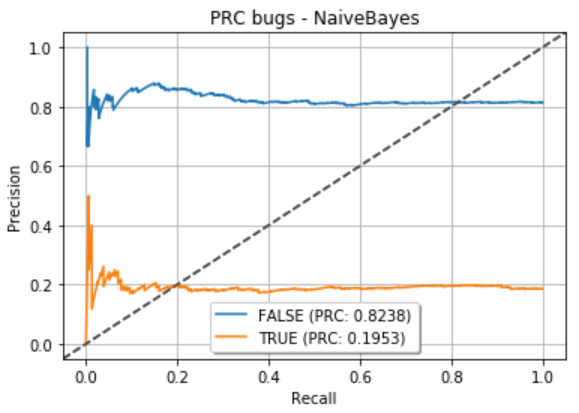
\includegraphics[width=2.7cm]{img/naive.PNG}
  \caption{Naive Bayes - PRC Curve}
  \label{fig:sub1}
\end{subfigure}
\begin{subfigure}{.3\linewidth}
  \centering
  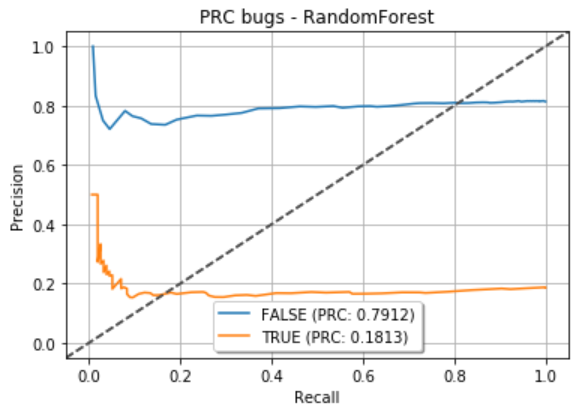
\includegraphics[width=2.7cm]{img/random_forest.PNG}
  \caption{Random Forest - PRC Curve}
  \label{fig:sub1}
\end{subfigure}
\begin{subfigure}{.3\linewidth}
  \centering
  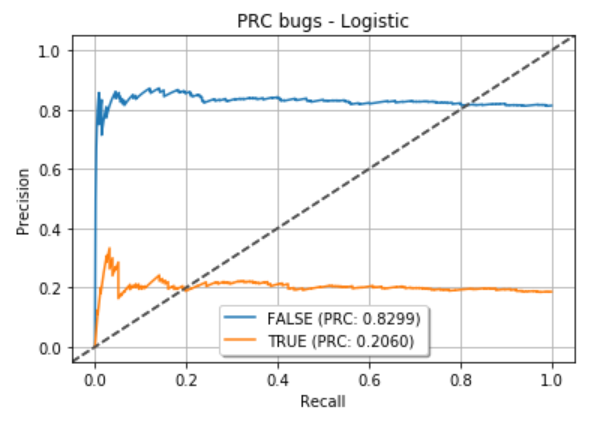
\includegraphics[width=2.7cm]{img/logistic.PNG}
  \caption{Logistic - PRC Curve}
  \label{fig:sub2}
\end{subfigure}
\caption{Precision - Recall Graphs}
\label{fig.aug}
\end{figure} 

\begin{center}
 \begin{tabular}{||c c c c||} 
 \hline
 ML Algorithm &Precision & Recall & F Score   \\ [0.5ex] 
 \hline\hline
  Naive Bayes &0.210526&0.025641& 0.045714\\ 
 \hline
 Random Forest & 0.238095 & 0.032051 & 0.056497 \\
 \hline
 Logistic & Nan & 0.0 & Nan \\
 \hline

\end{tabular}

\end{center}

According to the precision recall graphs, it is observed that all 3 types of prediction models were poorly performed with the given data due to the not having enough data to train the model. 

As a solution, with the intention of improving the size of the data set, data collected through 10 releases were concatenated together before feeding in to each prediction model. Observed results showed improvement in results compared to the existing performances. Improvement in the results of Random Forest prediction model was highly significant. 

\vspace{0.5cm}
Training Data - 
Non Defects Classes - 2013, Defect Classes - 893

\vspace{0.5cm}
\begin{figure}[h] 
\centering
\captionsetup{justification=centering}
\begin{subfigure}{.3\linewidth}
  \centering
  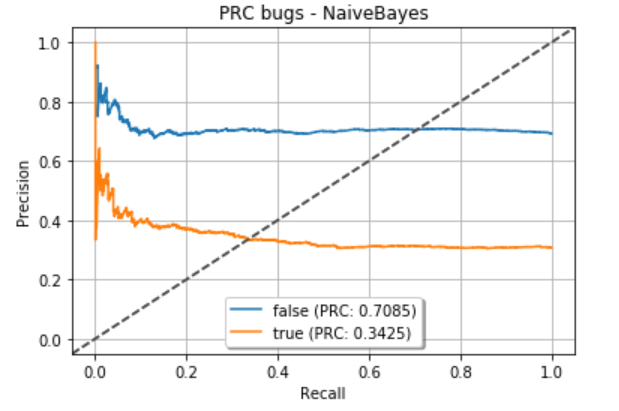
\includegraphics[width=2.7cm]{img/naive_10.PNG}
  \caption{Naive Bayes - PRC Curve}
  \label{fig:sub1}
\end{subfigure}
\begin{subfigure}{.3\linewidth}
  \centering
  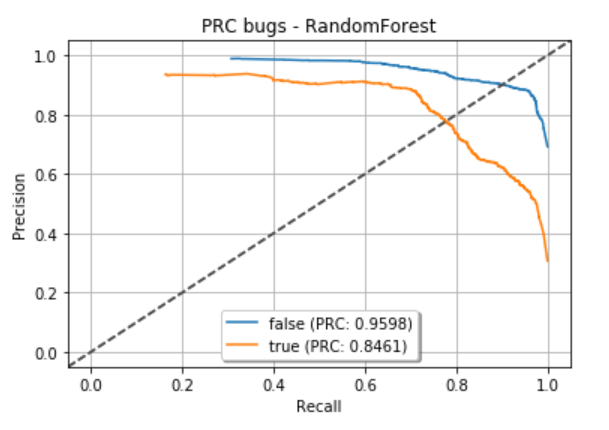
\includegraphics[width=2.7cm]{img/random_forest_10.PNG}
  \caption{Random Forest - PRC Curve}
  \label{fig:sub1}
\end{subfigure}
\begin{subfigure}{.3\linewidth}
  \centering
  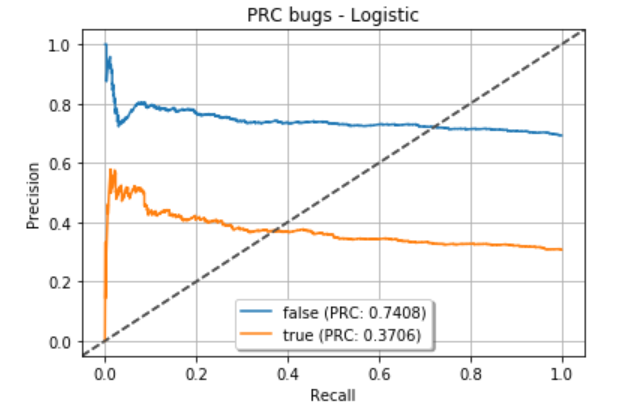
\includegraphics[width=2.7cm]{img/logistic_10.PNG}
  \caption{Logistic - PRC Curve}
  \label{fig:sub2}
\end{subfigure}
\caption{Precision - Recall Graphs}
\label{fig.aug}
\end{figure} 
\begin{center}
 \begin{tabular}{||c c c c||} 
 \hline
 ML Algorithm &Precision & Recall & F Score   \\ [0.5ex] 
 \hline\hline
  Naive Bayes &0.3070136&0.818589& 0.446548\\ 
 \hline
 Random Forest & 0.811664 & 0.748040 & 0.778554 \\
 \hline
 Logistic & 0.024636 & 0.5 & 0.046958 \\
 \hline

\end{tabular}

\end{center}
 
After efficient analysis on data, it is witnessed that increment of the data size shows an increase of the performance. Random forest prediction model performed the best among all other prediction models with a highest F-measure.

Moving from more generalized version to cloud specific bug prediction, following keywords were considered to filter defect classes from commits.
Non Defects Classes - 3988, Defect Classes - 1893


Data Imbalance Technique "imblearn.oversampling.SMOTE" was performed on data set to over-sampling minority data.
\vspace{0.5cm}
\begin{figure}[H]
\centering
    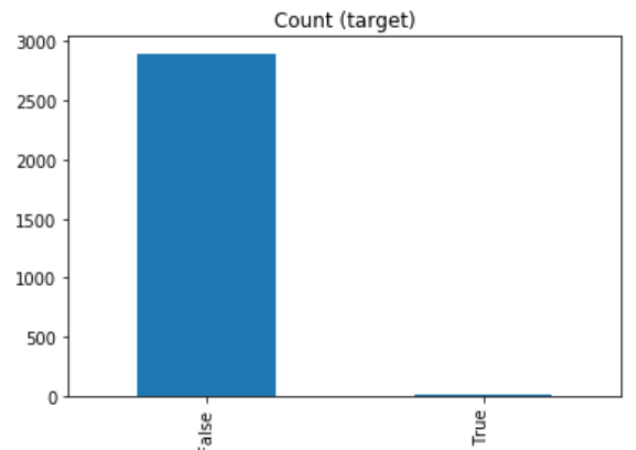
\includegraphics[width=0.4\textwidth]{img/Data_Imbalance_Cloud_Specific_Bugs.PNG}
    \caption{Data Imbalance - Cloud Specific Bugs}
    \label{fig:perc-cloudapps-categories}
\end{figure}
\vspace{0.5cm}
\begin{itemize}
\item "distributed concurrency","performance","single-point-of-failure"
\end{itemize}
\vspace{0.5cm}



Training Data - Non Defects Classes - 3988, Defect Classes - 1893

\vspace{0.5cm}
\begin{figure}[h] 
\centering
\captionsetup{justification=centering}
\begin{subfigure}{.3\linewidth}
  \centering
  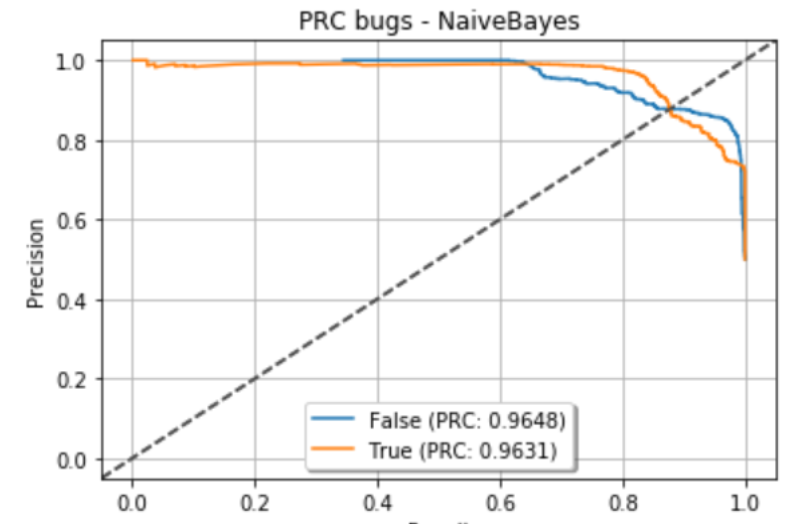
\includegraphics[width=2.7cm]{img/naive_cloud_specific.PNG}
  \caption{Naive Bayes - PRC Curve}
  \label{fig:sub1}
\end{subfigure}
\begin{subfigure}{.3\linewidth}
  \centering
  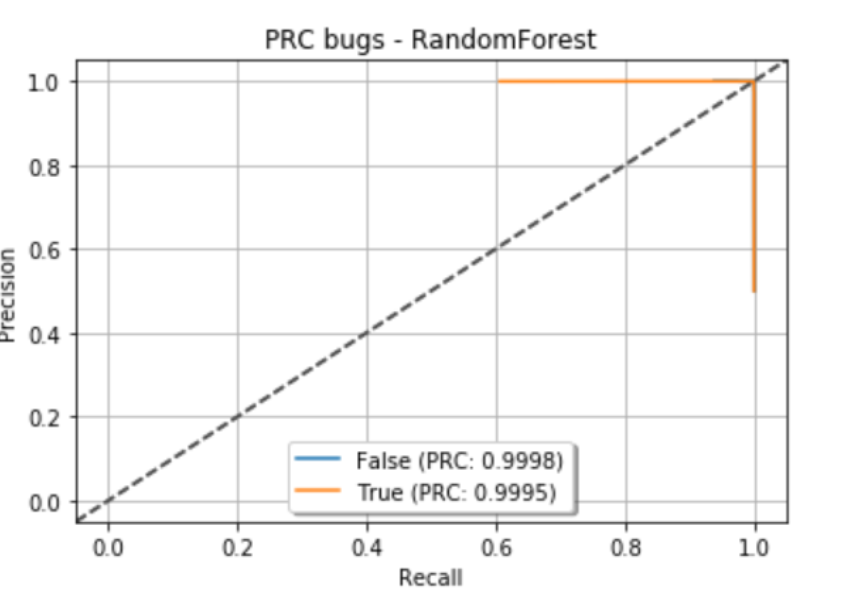
\includegraphics[width=2.7cm]{img/random_forest_cloud_specific.PNG}
  \caption{Random Forest - PRC Curve}
  \label{fig:sub1}
\end{subfigure}
\begin{subfigure}{.3\linewidth}
  \centering
  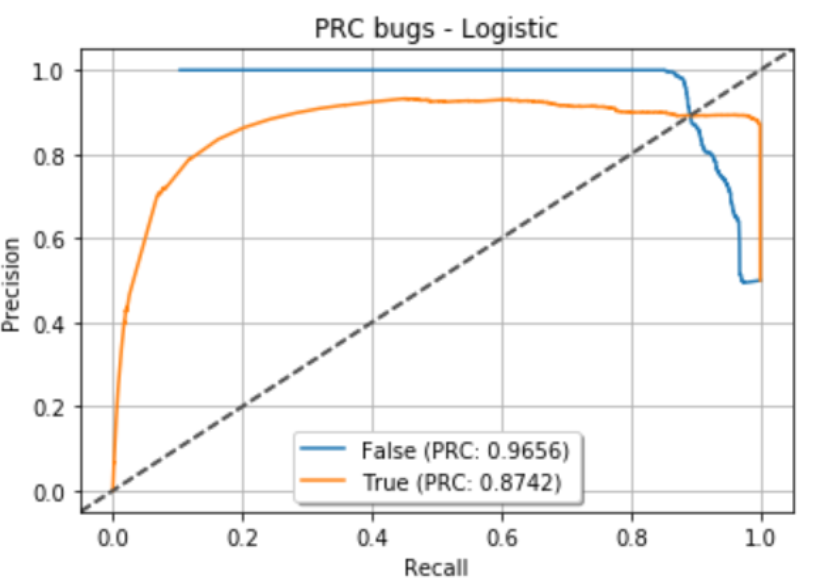
\includegraphics[width=2.7cm]{img/logistic_cloud_speicific.PNG}
  \caption{Logistic - PRC Curve}
  \label{fig:sub2}
\end{subfigure}
\caption{Precision - Recall Graphs}
\label{fig.aug}
\end{figure} 
\begin{center}
 \begin{tabular}{||c c c c||} 
 \hline
 ML Algorithm &Precision & Recall & F Score   \\ [0.5ex] 
 \hline\hline
  Naive Bayes & 0.73876 & 0.99172 & 0.84675\\ 
 \hline
 Random Forest & 0.99690 & 0.99965 & 0.99827 \\
 \hline
 Logistic & 0.88265 & 0.99344 & 0.93478 \\
 \hline
\end{tabular}

\end{center}
\vspace{0.5cm}

Then we tried to perform same experiment procedure for all types of cloud bugs we found.

\vspace{0.5cm}
Cloud concurrency bugs

\begin{itemize}
\item  'blocked', 'locked', 'race', 'dead-lock', 'deadlock', 'atomic','starvation', 'suspension', 'order violation', 'atomicity violation', 'single variable atomicity violation', 'multi variable atomicity violation', 'livelock',  'live-lock'
\end{itemize}


\vspace{0.5cm}
\begin{figure}[h] 
\centering
\captionsetup{justification=centering}
\begin{subfigure}{.3\linewidth}
  \centering
  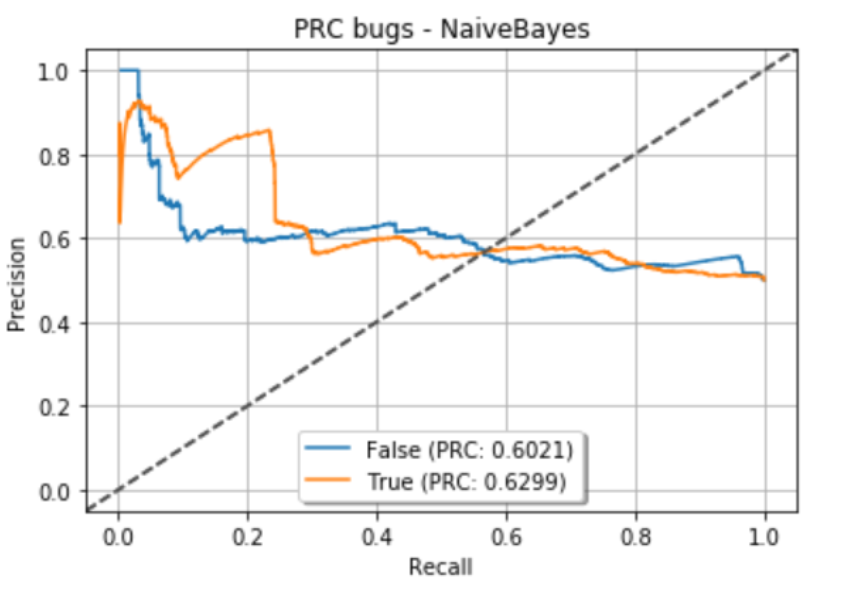
\includegraphics[width=2.7cm]{img/naive_cloud_concurrent.PNG}
  \caption{Naive Bayes - PRC Curve}
  \label{fig:sub1}
\end{subfigure}
\begin{subfigure}{.3\linewidth}
  \centering
  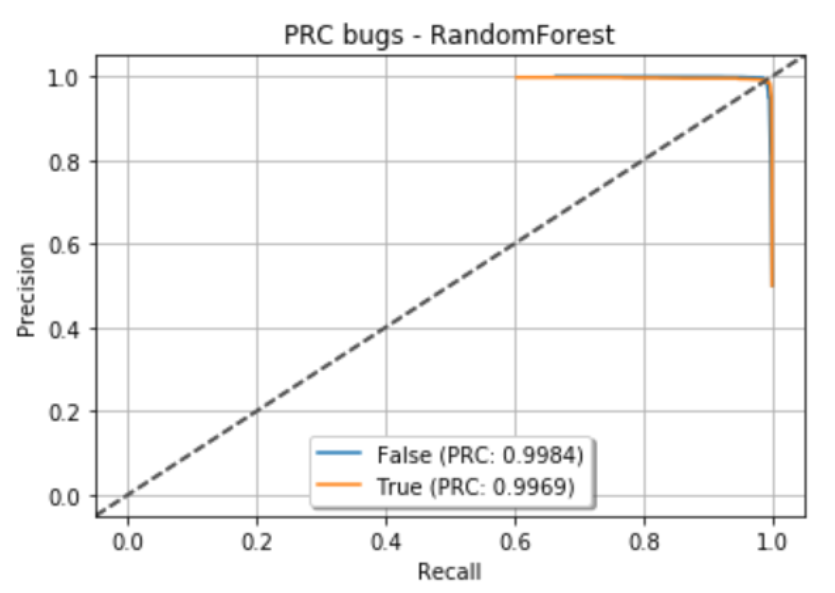
\includegraphics[width=2.7cm]{img/random_forest_cloud_concurrency.PNG}
  \caption{Random Forest - PRC Curve}
  \label{fig:sub1}
\end{subfigure}
\begin{subfigure}{.3\linewidth}
  \centering
  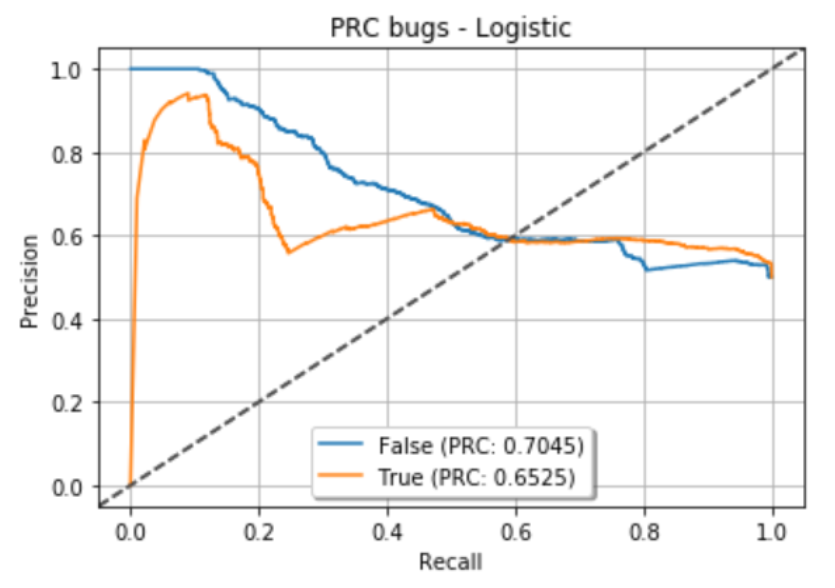
\includegraphics[width=2.7cm]{img/logistic_cloud_concurrency.PNG}
  \caption{Logistic - PRC Curve}
  \label{fig:sub2}
\end{subfigure}
\caption{Precision - Recall Graphs}
\label{fig.aug}
\end{figure} 
\begin{center}
 \begin{tabular}{||c c c c||} 
 \hline
 ML Algorithm &Precision & Recall & F Score   \\ [0.5ex] 
 \hline\hline
  Naive Bayes & 0.51747 & 0.90544 & 0.65857\\ 
 \hline
 Random Forest &  0.98572 & 0.99507 & 0.99037 \\
 \hline
 Logistic & 0.64829 & 0.47557 & 0.54866 \\
 \hline
\end{tabular}
\end{center}

\vspace{0.5cm}
Performance bugs

\begin{itemize}
\item  'performance','load balancing','cloud bursting', 'performance implications'
\end{itemize}


\vspace{0.5cm}
\begin{figure}[h] 
\centering
\captionsetup{justification=centering}
\begin{subfigure}{.3\linewidth}
  \centering
  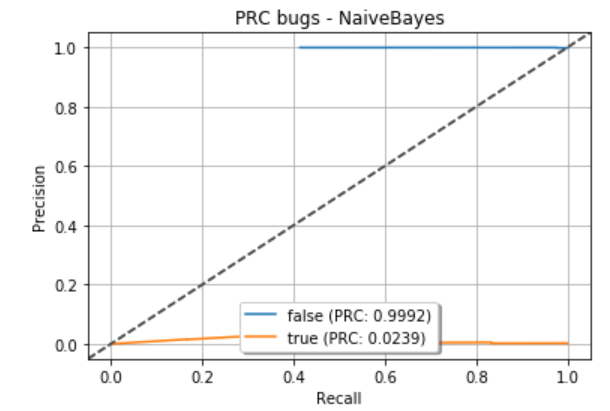
\includegraphics[width=2.7cm]{img/naive_prc.PNG}
  \caption{Naive Bayes - PRC Curve}
  \label{fig:sub1}
\end{subfigure}
\begin{subfigure}{.3\linewidth}
  \centering
  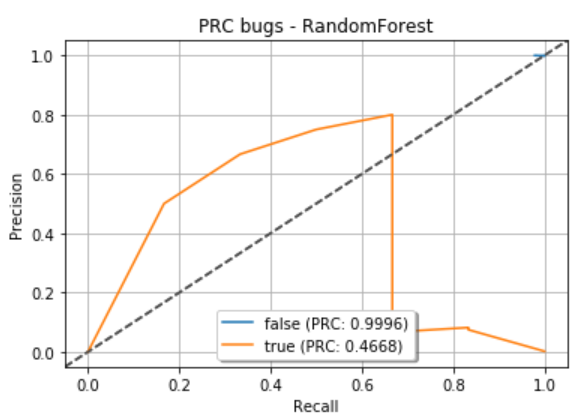
\includegraphics[width=2.7cm]{img/random_forest_performance.PNG}
  \caption{Random Forest - PRC Curve}
  \label{fig:sub1}
\end{subfigure}
\begin{subfigure}{.3\linewidth}
  \centering
  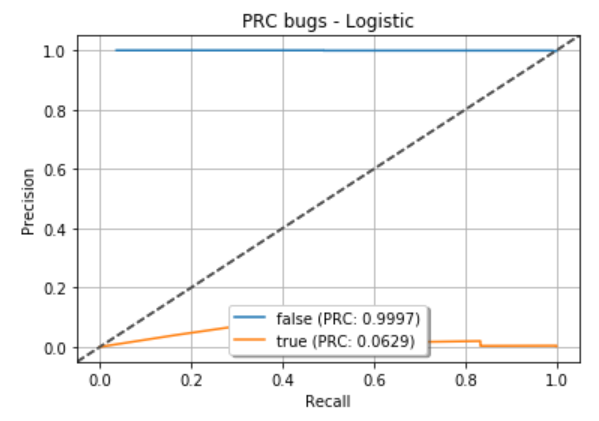
\includegraphics[width=2.7cm]{img/logistic_performance.PNG}
  \caption{Logistic - PRC Curve}
  \label{fig:sub2}
\end{subfigure}
\caption{Precision - Recall Graphs}
\label{fig.aug}
\end{figure} 
\begin{center}
 \begin{tabular}{||c c c c||} 
 \hline
 ML Algorithm &Precision & Recall & F Score   \\ [0.5ex] 
 \hline\hline
  Naive Bayes & 0.00740 & 0.666666 & 0.014652\\ 
 \hline
 Random Forest &  0.8 & 0.66666 & 0.72727 \\
 \hline
 Logistic & 0.0 & 0.0 & 0.0 \\
 \hline
\end{tabular}
\end{center}

\vspace{0.5cm}
Error Handling bugs

\begin{itemize}
\item  'error handling', 'exception', 'exceptions'
\end{itemize}



\vspace{0.5cm}
\begin{figure}[h] 
\centering
\captionsetup{justification=centering}
\begin{subfigure}{.3\linewidth}
  \centering
  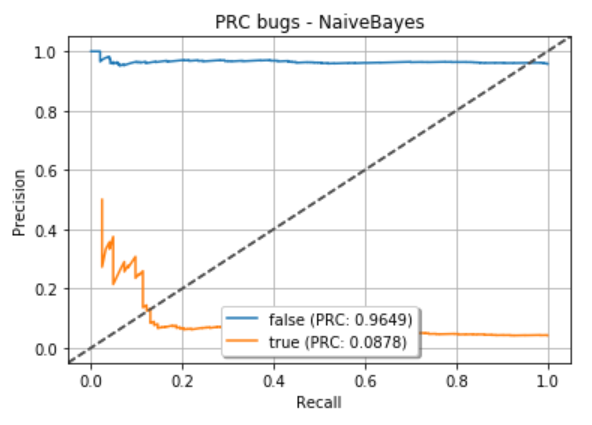
\includegraphics[width=2.7cm]{img/naive_error_handling.PNG}
  \caption{Naive Bayes - PRC Curve}
  \label{fig:sub1}
\end{subfigure}
\begin{subfigure}{.3\linewidth}
  \centering
  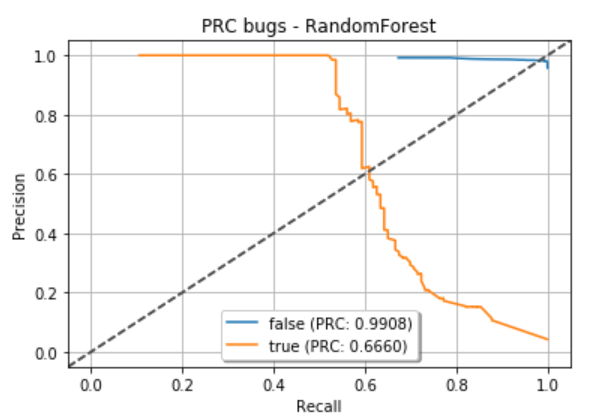
\includegraphics[width=2.7cm]{img/random_forest_error_handling.PNG}
  \caption{Random Forest - PRC Curve}
  \label{fig:sub1}
\end{subfigure}
\begin{subfigure}{.3\linewidth}
  \centering
  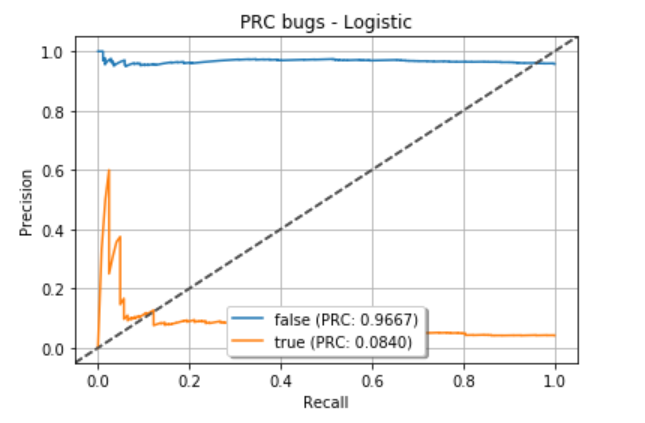
\includegraphics[width=2.7cm]{img/logistic_error_handling.PNG}
  \caption{Logistic - PRC Curve}
  \label{fig:sub2}
\end{subfigure}
\caption{Precision - Recall Graphs}
\label{fig.aug}
\end{figure} 
\begin{center}
 \begin{tabular}{||c c c c||} 
 \hline
 ML Algorithm &Precision & Recall & F Score   \\ [0.5ex] 
 \hline\hline
  Naive Bayes & 0.080568 & 0.138211 & 0.10179\\ 
 \hline
 Random Forest &  0.891891 & 0.536585 & 0.670050 \\
 \hline
 Logistic & 0.333333 & 0.008130 & 0.015873 \\
 \hline
\end{tabular}
\end{center}
\vspace{0.5cm}
Configuration bugs

\begin{itemize}
\item  'configuration'
\end{itemize}

\vspace{0.5cm}
\begin{figure}[h] 
\centering
\captionsetup{justification=centering}
\begin{subfigure}{.3\linewidth}
  \centering
  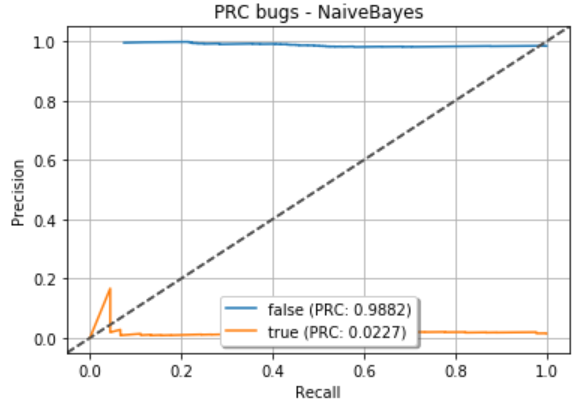
\includegraphics[width=2.7cm]{img/naive_configurations.PNG}
  \caption{Naive Bayes - PRC Curve}
  \label{fig:sub1}
\end{subfigure}
\begin{subfigure}{.3\linewidth}
  \centering
  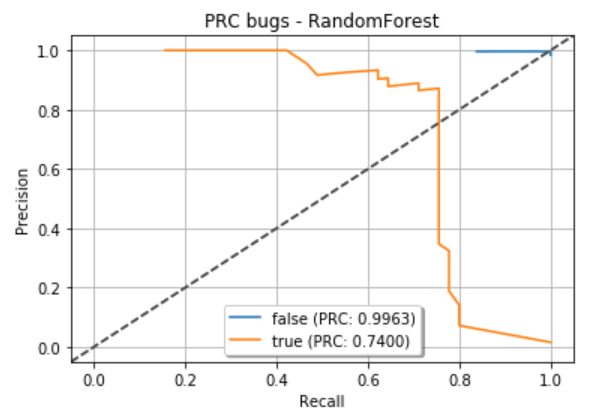
\includegraphics[width=2.7cm]{img/random_configuration.PNG}
  \caption{Random Forest - PRC Curve}
  \label{fig:sub1}
\end{subfigure}
\begin{subfigure}{.3\linewidth}
  \centering
  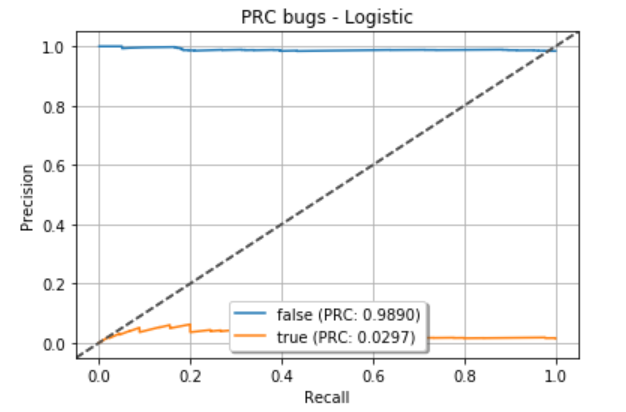
\includegraphics[width=2.7cm]{img/logistic_configuration.PNG}
  \caption{Logistic - PRC Curve}
  \label{fig:sub2}
\end{subfigure}
\caption{Precision - Recall Graphs}
\label{fig.aug}
\end{figure} 
\begin{center}
 \begin{tabular}{||c c c c||} 
 \hline
 ML Algorithm &Precision & Recall & F Score   \\ [0.5ex] 
 \hline\hline
  Naive Bayes & 0.01276 & 0.355555 & 0.024653\\ 
 \hline
 Random Forest &  0.790123 & 0.888888 & 0.711111 \\
 \hline
 Logistic & 0.0 & 0.0 & 0.0 \\
 \hline
\end{tabular}
\end{center}
\vspace{0.5cm}

One other important issue we witnessed was, not having enough data for classifying as defect classes. Even we used re sampling method to over sample data, observed results graphs shows some strange behaviour due to resampling. 

Apart from that,we cant generalize this to all the cloud projects without extensive analysis on different cloud projects. But still experiment should be extended to carry out on improving sample size of each type of bugs.


\subsection{RQ2: ASAT Adoption}
In our sample, cloud projects use on average 12.5 ASATs whereas non-cloud projects only use 5.0. Breaking down those total numbers by category, we get the following numbers:\\

Cloud projects:
\begin{itemize}
    \item None:  1.3
    \item Correctness:  1.7
    \item Readability:  5.5
    \item Efficiency:  3.7
    \item Security:  0.2
\end{itemize}

Non-cloud projects:
\begin{itemize}
    \item None:  0.5
    \item Correctness:  0.7
    \item Readability:  2.3
    \item Efficiency:  1.5
    \item Security: 0.0
\end{itemize}

Figures \ref{fig:perc-cloudapps} and \ref{fig:perc-noncloudapps} show the percentages of cloud and non-cloud projects using a given ASAT. As can be seen from the figures, some ASATs are not used in any of the projects such as 'safesql' (SQL injections) or 'dingo-hunter' (deadlocks). Most commonly used are 'unused' (unused code), 'govet' (code correctness) and 'gofmt' (code formatting) (>=70\%). Cloud projects use every ASAT at least as frequently as non-cloud projects. Thus, there is no ASAT that is more common in non-cloud projects than in cloud projects. On the other hand, there are quite a few ASATs that are ran more often in cloud projects than in non-cloud projects (i.e. at least 20\% difference):

\begin{itemize}
    \item wsl (empty lines): 8 vs. 33 \%
    \item unused (unused code): 42 vs. 93 \%
    \item unconvert (unnecessary type conversions): 0 vs. 27 \%
    \item misspell (misspellings): 25 vs. 93 \%
    \item ineffassign (ineffectual assignments): 17 vs. 60 \%
    \item govet (code correctness): 58 vs. 87 \%
    \item gosimple (simplifying code): 17 vs. 40 \%
    \item gosec (security issues): 0 vs. 20 \%
    \item golint (coding style issues): 33 vs. 80 \%
    \item goimports (package import issues): 8 vs. 73 \%
    \item gofmt (formatting issues): 50 vs. 93 \%
    \item errcheck (error return values): 42 vs. 73 \%
    \item deadcode (unused code): 17 vs. 60 \%
\end{itemize}


\begin{figure}
\centering
    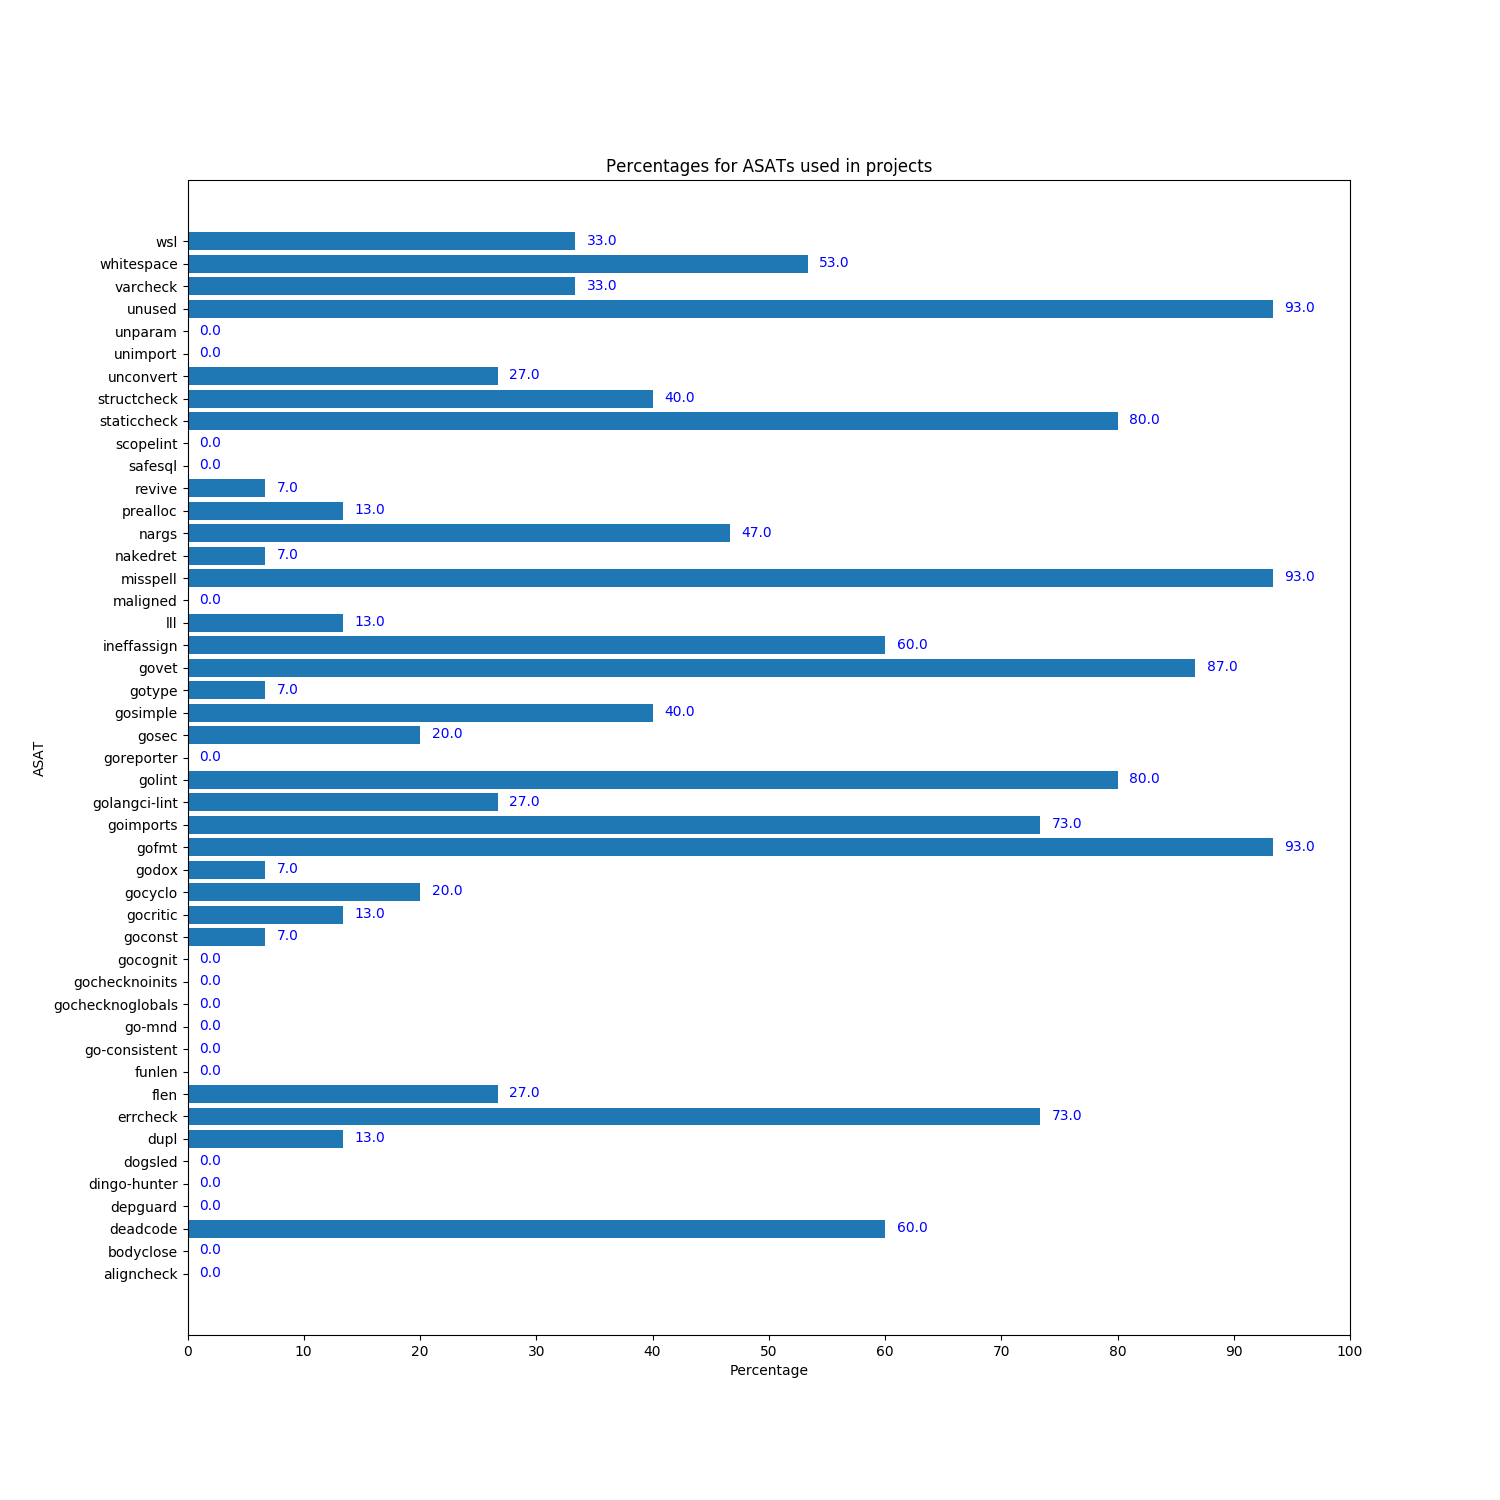
\includegraphics[width=0.6\textwidth]{img/cloud-projects.png}
    \caption{Percentages of cloud projects using a given ASAT.}
    \label{fig:perc-cloudapps}
\end{figure}

\begin{figure}
\centering
    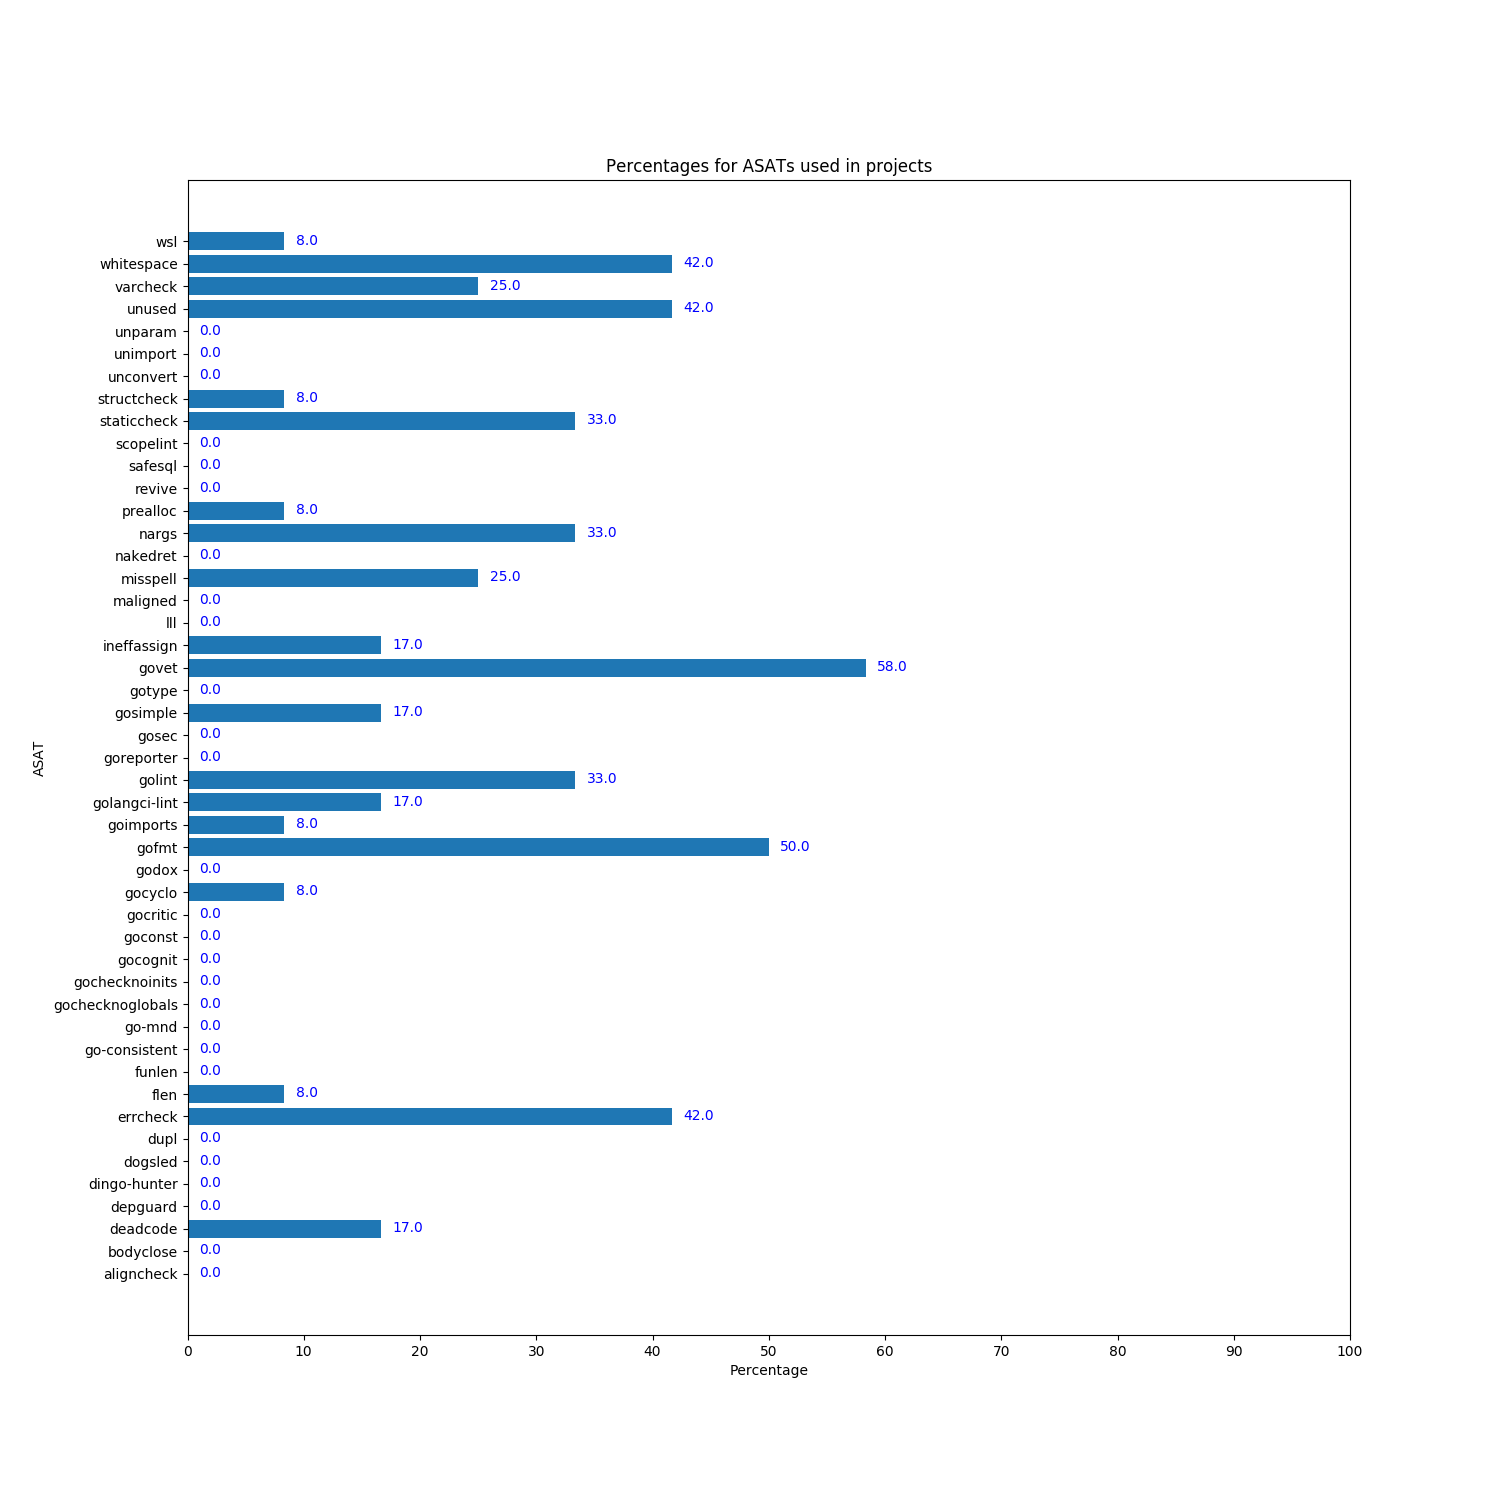
\includegraphics[width=0.6\textwidth]{img/non-cloud-projects.png}
    \caption{Percentages of non-cloud projects using a given ASAT.}
    \label{fig:perc-noncloudapps}
\end{figure}

Figures \ref{fig:perc-cloudapps-categories} and \ref{fig:perc-noncloudapps-categories} show the percentages of cloud and non-cloud projects using a given ASAT category. As can be observed from the figures, security linters are rarely used -- in non-cloud projects not at all and in cloud projects in 20\% of the projects. On the other hand, the other categories of linters are much more often used. In fact, the cloud projects in our sample almost always use some sort of linter that checks for readability, correctness and efficiency issues. Non-cloud projects also use readability checkers often and sometimes efficiency and correctness checkers.

\begin{figure}
\centering
    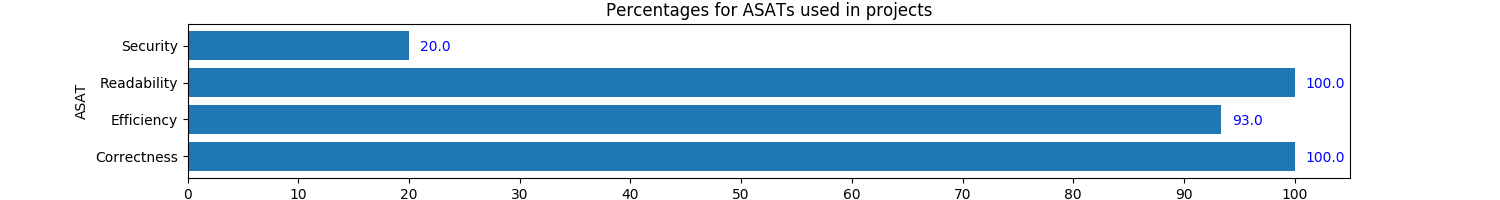
\includegraphics[width=0.6\textwidth]{img/cloud-projects-categories.png}
    \caption{Percentages of cloud projects using a given ASAT category.}
    \label{fig:perc-cloudapps-categories}
\end{figure}

\begin{figure}
\centering
    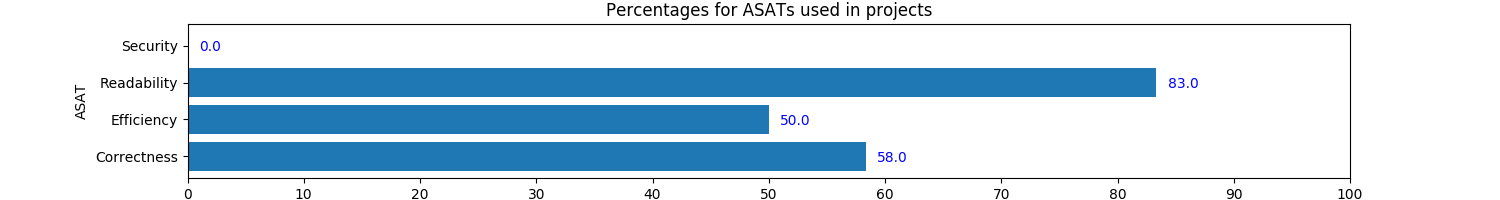
\includegraphics[width=0.6\textwidth]{img/non-cloud-projects-categories.png}
    \caption{Percentages of non-cloud projects using a given ASAT category.}
    \label{fig:perc-noncloudapps-categories}
\end{figure}

Regarding configuration of ASATs, cloud projects use the standard configuration in 65.8 \% of the cases, while non-cloud projects do so in 68.3 \% of the cases. Generally, most configuration options are rarely used and do not enable/disable warnings. Indeed, most options are about specifying which files/packages to run the linter on or how the warnings should be output.


\section{Threats to Validity}
\begin{itemize}
    \item Our project sample is rather small and only contains large projects. Therefore, our results might not generalize well when considering more projects or smaller projects.
    \item One author only classified the ASATs. These classifications might be subjective. Other people might classify them differently.
    \item The code might contain bugs that might affect our results. We do not have comprehensive set of automated tests. Instead we manually inspected the code output.
    \item Use selected keywords are not the optimal set of keywords for filtering bugs. 
    \item Due to limited time it wasnt possible for us to manual check all the filtered commits to identify the validity of using keywords.
\end{itemize}

\section{Conclusion and Future Work}
We conducted two different experiments to investigate how bug prediction and ASAT adoption works for cloud applications.

In the case of using machine learning pipeline for bug prediction we tried to specialize by feeding only cloud specific bugs. Experiment was carried out only for one cloud project "Hadoop" and in the future we plan to increase the sample project size and analyse the performance to get a better idea on the results. 
In the current context, commit filtering was done using manually selected keywords and next step of the project is to use natural language processing help on commit filtering. 

Complement to filtering bugs through keywords, from recent studies it is observed that analysing system log of the cloud environment would be a better choice to find defected modules but from higher architecture level except of class level.

Regarding ASAT adoption, we found that cloud applications use more and a larger variety of ASATs than non-cloud applications. Typically, both kinds of projects use the default configuration of the ASATs.

In the future, we plan to increase our sample size. We also want to experiment with other features for bug prediction. Moreover, to make our code more robust and bug-free, we will write some automated tests. Furthermore, we will involve a second person for classifying the ASATs and determine whether inter-rater agreement is good enough to accept the classifications.

%\begin{lstlisting}[caption=An example code snippet]
%/**
% * Javadoc comment
% */
%public class Foo {
%	// line comment
%	public void bar(int number) {
%		if (number < 0) {
%			return; /* block comment */
%		}
%	}
%}
%\end{lstlisting}

\bibliographystyle{abbrv}
\bibliography{references}

\end{document}
